\documentclass[a4paper,12pt]{article}
\newcommand{\cName}{Jenish Pant} % Name of the student
\newcommand{\cRollNo}{THA078BEI018} % Roll no. of the student
\newcommand{\cSubj}{Computer Network} % Subject
\newcommand{\cLabNumber}{5}
\newcommand{\cSubmissionDate}{\today} % Submission date
\newcommand{\cTitle}{STATIC ROUTING IN CISCO PACKET TRACER}
\title{Lab5: Setting up Static Routing in Cisco Packet Tracer}
\author{\cName}

\usepackage{graphicx} % For including images
\usepackage{amsmath} % For better math support
\usepackage[a4paper]{geometry}

\geometry{
  textwidth=\dimexpr\paperwidth-29mm,
  textheight=\dimexpr\paperheight-32mm,
  noheadfoot,
  nomarginpar
}

\setlength{\topskip}{0mm}
\setlength{\parindent}{0mm}

\title{Lab \cLabNumber: \cTitle}
\date{}
\author{}
\begin{document}

\maketitle
\vspace{-2cm}
\section*{INTRODUCTION}
In this laboratory session, we investigate the setup and execution of static routing using Cisco Packet Tracer. Static routing, a basic networking principle, involves manually defining routes by the network administrator. The purpose of this lab is to offer practical exposure to configuring static routes, grasping their significance, and assessing network behavior to facilitate efficient communication in a specified network layout.

\section*{OBJECTIVES}
\begin{itemize}
    \item To understand the concept of static routing in a network.
    \item To configure static routes on routers in a network topology.
    \item To analyze the network behavior and verify connectivity between hosts.
\end{itemize}

\section*{THEORY}

\subsubsection*{Static Routing}
Static routing is a type of network routing technique in which routes are manually configured by a network administrator using route entries. Unlike dynamic routing, static routing does not use routing protocols to determine the best path for data packets. Instead, it relies on the predefined path set by the administrator. Static routes are useful for small networks or for specific routing needs where the routes do not change frequently.

\section*{LAB SETUP}
\subsection{Network Topology}
The network topology for this lab consists of three routers, two switches, and four PCs. The layout is as follows:
\begin{itemize}
    \item \textbf{Router1} is connected to \textbf{Router2} and \textbf{Router3}.
    \item \textbf{Router2} is connected to \textbf{Router1} and \textbf{Router3}.
    \item \textbf{Router1} is connected to \textbf{Switch1}.
    \item \textbf{Router3} is connected to \textbf{Switch2}.
    \item \textbf{Switch1} connects two PCs (\textbf{PC1} and \textbf{PC2}).
    \item \textbf{Switch2} connects two PCs (\textbf{PC3} and \textbf{PC4}).
\end{itemize}

\begin{figure}[h!]
    \centering
    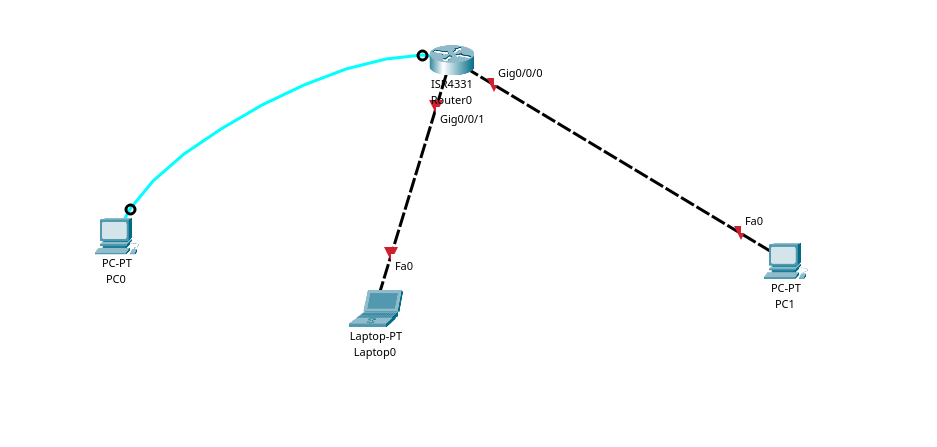
\includegraphics[width=0.8\textwidth]{img/topology.png}
    \caption{Network Topology}
\end{figure}

\subsection*{IP Subnetting}
The given network address is 192.169.0.0/24. We will divide this network into five subnets as required by the network topology. The subnets consists of following number of hosts:
\begin{itemize}
    \item \textbf{Subnet 1}: 30 hosts
    \item \textbf{Subnet 2}: 16 hosts
    \item \textbf{Subnet 3}: 2 hosts
    \item \textbf{Subnet 4}: 2 hosts
    \item \textbf{Subnet 5}: 2 hosts
\end{itemize}

\begin{table}[h!]
    \centering
    \caption{IP Subnetting Table}
    \begin{tabular}{lccc}
        \toprule
        \textbf{Subnet} & \textbf{Network Address} & \textbf{Subnet Mask} & \textbf{Host Range}         \\
        \midrule
        N1              & 192.168.0.0/24           & 255.255.255.224      & 192.168.0.1 - 192.168.0.30  \\
        N2              & 192.168.0.32/28          & 255.255.255.240      & 192.168.0.33 - 192.168.0.40 \\
        N3              & 192.168.0.48/30          & 255.255.255.252      & 192.168.0.49 - 192.168.0.50 \\
        N4              & 192.168.0.52/30          & 255.255.255.252      & 192.168.0.53 - 192.168.0.54 \\
        N5              & 192.168.0.56/30          & 255.255.255.252      & 192.168.0.57 - 192.168.0.58 \\
        \bottomrule
    \end{tabular}
\end{table}


\subsection*{Static Routing Configuration}
To enable communication between all devices in the network, static routes need to be configured on each router. These routes ensure that data packets are directed to their appropriate destinations. The following configurations are applied to each router:

\subsection*{Router1 Configuration}
\begin{verbatim}
    Router1(config)# ip route 192.168.0.32 255.255.255.240 192.168.0.50
    Router1(config)# ip route 192.168.0.56 255.255.255.252 192.168.0.54
    \end{verbatim}

\subsection*{Router2 Configuration}
\begin{verbatim}
    Router2(config)# ip route 192.168.0.0 255.255.255.224 192.168.0.53
    Router2(config)# ip route 192.168.0.48 255.255.255.252 192.168.0.53
    Router2(config)# ip route 192.168.0.32 255.255.255.240 192.168.0.57
    \end{verbatim}

\subsection*{Router3 Configuration}
\begin{verbatim}
    Router3(config)# ip route 192.168.0.0 255.255.255.224 192.168.0.49
    Router3(config)# ip route 192.168.0.48 255.255.255.252 192.168.0.58
\end{verbatim}



\section*{RESULTS}
After configuring the static routes on the routers, we verified the connectivity between the PCs in the network. The network was able to communicate successfully, and all devices were able to ping each other.




\begin{figure}[!h]
    \centering
    \begin{minipage}{0.45\textwidth}
        \centering
        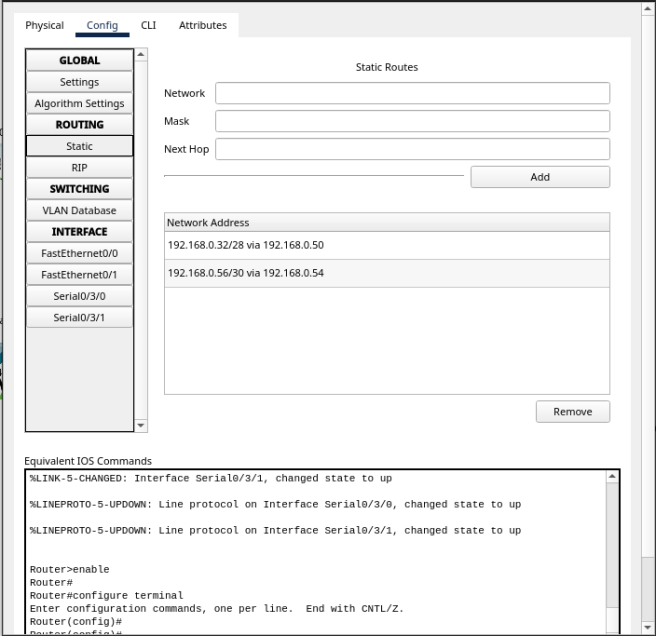
\includegraphics[width=\textwidth]{img/router1.png}
        \caption{Router 1 Static Routes}
    \end{minipage}\hfill
    \begin{minipage}{0.45\textwidth}
        \centering
        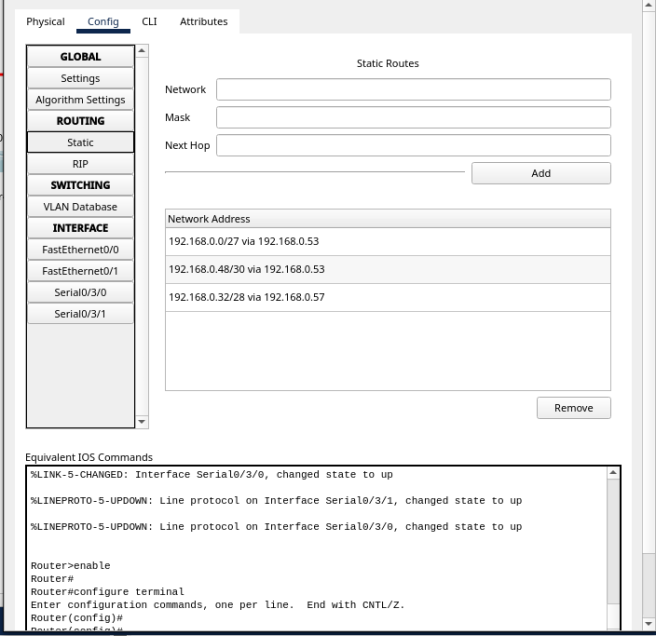
\includegraphics[width=\textwidth]{img/router2.png}
        \caption{Router 2 Static Routes}
    \end{minipage}
\end{figure}

\begin{figure}[h!]
    \centering
    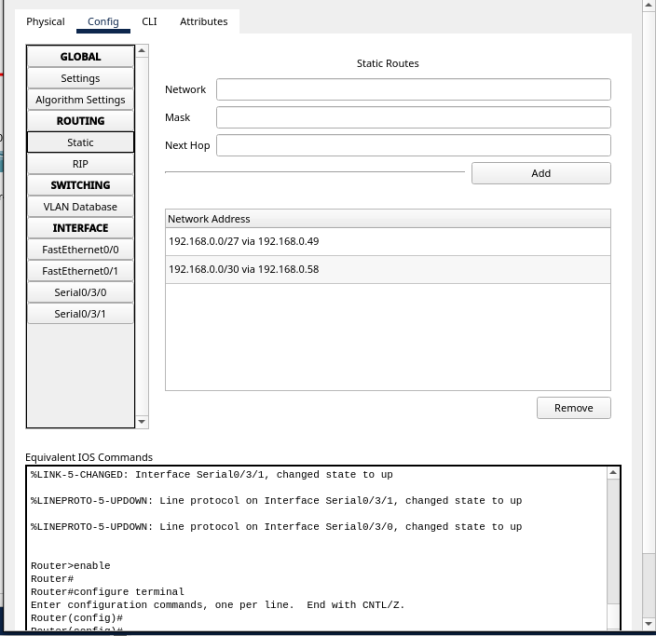
\includegraphics[width=0.4\textwidth]{img/router3.png}
    \caption{Router 3 Static Routes}
\end{figure}

\begin{figure}[h!]
    \centering
    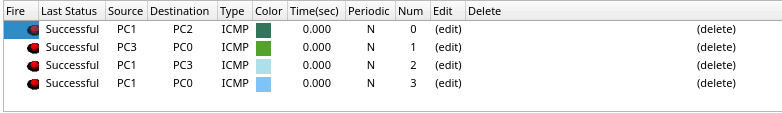
\includegraphics[width=0.8\textwidth]{img/ping.png}
    \caption{Ping Test Results}
\end{figure}

\newpage
\section*{CONCLUSION}
In this lab, we successfully configured static routes on a network topology using Cisco Packet Tracer. We learned the importance of static routing in directing data packets to their appropriate destinations. We also understood how static routes are manually configured by a network administrator. After setting up the network and configuring the routes, we were able to verify the connectivity between all devices in the network. All devices were able to communicate with each other successfully, demonstrating the effectiveness of our static routing configuration. This lab has provided us with practical experience and a deeper understanding of static routing in computer networks.
\end{document}
